%==============================================================
%  Task 2 — News Category Classification  |  AG News Dataset
%  LaTeX Beamer Presentation
%==============================================================
\documentclass[aspectratio=169,11pt]{beamer}
\usetheme{Madrid}
\usecolortheme{default}

\definecolor{primary}{RGB}{30,80,140}
\definecolor{accent}{RGB}{220,70,50}
\definecolor{light}{RGB}{240,245,252}
\definecolor{worldcol}{RGB}{78,121,167}
\definecolor{sportscol}{RGB}{220,130,40}
\definecolor{businesscol}{RGB}{200,70,70}
\definecolor{scitechcol}{RGB}{80,160,155}
\definecolor{darkgray}{RGB}{50,50,50}
\definecolor{greencol}{RGB}{60,160,80}

\setbeamercolor{palette primary}{bg=primary,fg=white}
\setbeamercolor{palette secondary}{bg=primary!80,fg=white}
\setbeamercolor{palette tertiary}{bg=primary!60,fg=white}
\setbeamercolor{palette quaternary}{bg=primary,fg=white}
\setbeamercolor{structure}{fg=primary}
\setbeamercolor{frametitle}{bg=primary,fg=white}
\setbeamercolor{block title}{bg=primary,fg=white}
\setbeamercolor{block body}{bg=light}
\setbeamercolor{alerted text}{fg=accent}

\usepackage[utf8]{inputenc}
\usepackage[T1]{fontenc}
\usepackage{amsmath,amssymb}
\usepackage{booktabs}
\usepackage{graphicx}
\usepackage{xcolor}
\usepackage{tikz}
\usetikzlibrary{shapes.geometric,arrows.meta,positioning,fit,calc,matrix}
\usepackage{pgfplots}
\pgfplotsset{compat=1.18}
\usepackage{array}
\usepackage{colortbl}
\usepackage{tcolorbox}
\tcbuselibrary{skins,breakable}

\newcommand{\highlight}[1]{\textcolor{accent}{\textbf{#1}}}

% TikZ style using #1 must be in preamble to avoid beamer "Illegal parameter number" error
\tikzset{
  mlplayer/.style={draw=#1,fill=#1!15,rounded corners=5pt,
    minimum width=1.8cm,minimum height=3.5cm,font=\small\bfseries,align=center}
}

\title[News Classification | AG News]{\textbf{News Category Classification}}
\subtitle{A Full Machine Learning Pipeline on the AG News Dataset}
\author{Text Classification Project}
\institute[NLP]{Natural Language Processing $\cdot$ Machine Learning}
\date{\today}

\begin{document}

%--- TITLE ---
\begin{frame}[plain]
    \vspace{1cm}
\begin{tikzpicture}[remember picture,overlay]
  \fill[primary] (current page.north west) rectangle (current page.south east);
  \filldraw[white,opacity=0.04] (current page.center) circle (6cm);
  \fill[worldcol]    ([yshift=0.55cm]current page.south west) rectangle ++(0.25\paperwidth,0.55cm);
  \fill[sportscol]   ([yshift=0.55cm,xshift=0.25\paperwidth]current page.south west) rectangle ++(0.25\paperwidth,0.55cm);
  \fill[businesscol] ([yshift=0.55cm,xshift=0.50\paperwidth]current page.south west) rectangle ++(0.25\paperwidth,0.55cm);
  \fill[scitechcol]  ([yshift=0.55cm,xshift=0.75\paperwidth]current page.south west) rectangle ++(0.25\paperwidth,0.55cm);
  \node[white,font=\small\bfseries] at ([yshift=0.825cm,xshift=0.125\paperwidth]current page.south west) {World};
  \node[white,font=\small\bfseries] at ([yshift=0.825cm,xshift=0.375\paperwidth]current page.south west) {Sports};
  \node[white,font=\small\bfseries] at ([yshift=0.825cm,xshift=0.625\paperwidth]current page.south west) {Business};
  \node[white,font=\small\bfseries] at ([yshift=0.825cm,xshift=0.875\paperwidth]current page.south west) {Sci/Tech};
  \node[white,font=\Huge\bfseries,text width=13cm,align=center] at ([yshift=1.5cm]current page.center) {News Category Classification};
  \node[white!80,font=\large,text width=12cm,align=center] at ([yshift=0.4cm]current page.center) {A Full ML Pipeline on the AG News Dataset};
  \node[white!60,font=\normalsize,text width=13cm,align=center] at ([yshift=-0.55cm]current page.center) {Logistic Regression $\cdot$ Linear SVM $\cdot$ Random Forest $\cdot$ MLP Neural Network};
  \node[white!45,font=\small] at ([yshift=-1.3cm]current page.center) {TF-IDF Feature Engineering $\cdot$ 120{,}000 Training Articles $\cdot$ 4 Categories};
\end{tikzpicture}
\end{frame}

%--- TOC ---
\begin{frame}{Outline}
\begin{columns}
  \column{0.55\textwidth}
    \tableofcontents[hideallsubsections]
  \column{0.42\textwidth}
    \begin{tcolorbox}[colback=light,colframe=primary,title=Quick Facts,fonttitle=\small\bfseries]
      \small
      \textbullet\ \textbf{120K} training articles\\[3pt]
      \textbullet\ \textbf{7,600} test articles\\[3pt]
      \textbullet\ \textbf{4} balanced categories\\[3pt]
      \textbullet\ TF-IDF + 4 classifiers\\[3pt]
      \textbullet\ Best accuracy \highlight{91.82\%}
    \end{tcolorbox}
\end{columns}
\end{frame}

\section{Introduction \& Dataset}

%--- Task Overview ---
\begin{frame}{Task Overview}
\begin{columns}[T]
  \column{0.55\textwidth}
  \vspace{-0.5cm}
    \begin{block}{Problem Statement}
      Automatically assign a \textbf{news article} to one of four topical categories using classical ML and a shallow neural network.
    \end{block}
    \vspace{1pt}
    \begin{block}{Pipeline Steps}
      \small
      \begin{enumerate}
        \item Load \& explore AG News dataset
        \item Text preprocessing (NLP pipeline)
        \item TF-IDF feature extraction
        \item Train 3 classical classifiers
        \item \textit{Bonus:} MLP Neural Network
        \item Evaluation \& visualisations
        \item \textit{Bonus:} Word clouds per category
      \end{enumerate}
    \end{block}
  \column{0.42\textwidth}
    \vspace{4pt}
    \begin{center}
    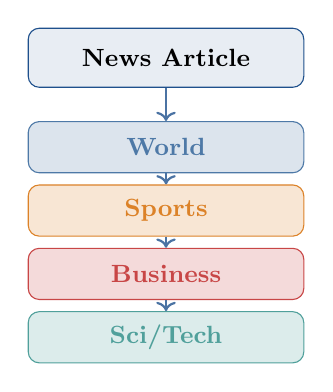
\begin{tikzpicture}
      \node[draw=primary,fill=primary!10,rounded corners,minimum width=3.5cm,minimum height=0.75cm,font=\small\bfseries] (inp) {News Article};
      \node[draw=worldcol,fill=worldcol!20,rounded corners,minimum width=3.5cm,minimum height=0.65cm,font=\small\bfseries,text=worldcol,below=12pt of inp] (w) {World};
      \node[draw=sportscol,fill=sportscol!20,rounded corners,minimum width=3.5cm,minimum height=0.65cm,font=\small\bfseries,text=sportscol,below=4pt of w] (s) {Sports};
      \node[draw=businesscol,fill=businesscol!20,rounded corners,minimum width=3.5cm,minimum height=0.65cm,font=\small\bfseries,text=businesscol,below=4pt of s] (b) {Business};
      \node[draw=scitechcol,fill=scitechcol!20,rounded corners,minimum width=3.5cm,minimum height=0.65cm,font=\small\bfseries,text=scitechcol,below=4pt of b] (t) {Sci/Tech};
      \draw[->,thick,primary!80] (inp) -- (w);
      \draw[->,thick,primary!80] (w) -- (s);
      \draw[->,thick,primary!80] (s) -- (b);
      \draw[->,thick,primary!80] (b) -- (t);
    \end{tikzpicture}
    \end{center}
\end{columns}
\end{frame}

%--- Dataset ---
\begin{frame}{AG News Dataset}
\begin{columns}[T]
  \column{0.50\textwidth}
    \begin{block}{Dataset at a Glance}
      \small
      \begin{itemize}
        \item Large-scale news topic classification benchmark
        \item Each sample: \textit{title} + \textit{description} combined
        \item 4 perfectly balanced categories (no class imbalance)
      \end{itemize}
    \end{block}
    \vspace{5pt}
    \begin{tcolorbox}[colback=light,colframe=primary,title=Split Summary,fonttitle=\footnotesize\bfseries]
      \centering\small
      \begin{tabular}{lrr}
        \toprule
        \textbf{Split} & \textbf{Articles} & \textbf{Per class}\\
        \midrule
        Train & 120,000 & 30,000 \\
        Test  & 7,600   & 1,900  \\
        \bottomrule
      \end{tabular}
    \end{tcolorbox}
  \column{0.47\textwidth}
    \begin{center}
    \textbf{Perfectly Balanced Classes}\\[6pt]
    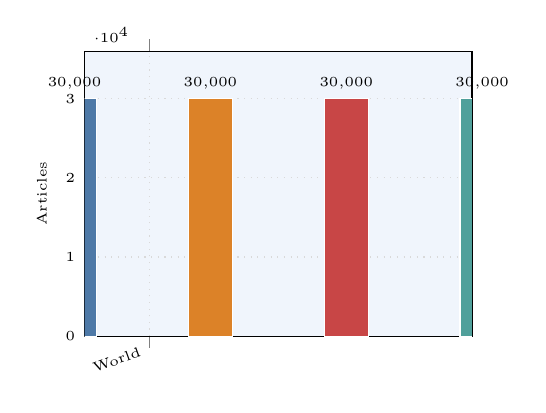
\begin{tikzpicture}
      \begin{axis}[
        ybar, bar width=16pt,
        width=6.5cm, height=5.2cm,
        symbolic x coords={World,Sports,Business,SciTech},
        xtick=data,
        xticklabels={World,Sports,Business,Sci/Tech},
        xticklabel style={font=\tiny,rotate=20,anchor=east},
        ymin=0, ymax=36000,
        ytick={0,10000,20000,30000},
        yticklabel style={font=\tiny},
        ylabel={Articles}, ylabel style={font=\tiny},
        nodes near coords, nodes near coords style={font=\tiny\bfseries},
        grid=major, grid style={dotted,gray!30},
        axis background/.style={fill=light},
        enlarge x limits=0.25,
      ]
        \addplot[fill=worldcol,draw=white]    coordinates {(World,30000)};
        \addplot[fill=sportscol,draw=white]   coordinates {(Sports,30000)};
        \addplot[fill=businesscol,draw=white] coordinates {(Business,30000)};
        \addplot[fill=scitechcol,draw=white]  coordinates {(SciTech,30000)};
      \end{axis}
    \end{tikzpicture}
    \end{center}
\end{columns}
\end{frame}

\section{Text Preprocessing}

%--- NLP Pipeline ---
\begin{frame}{Text Preprocessing Pipeline}
\begin{center}
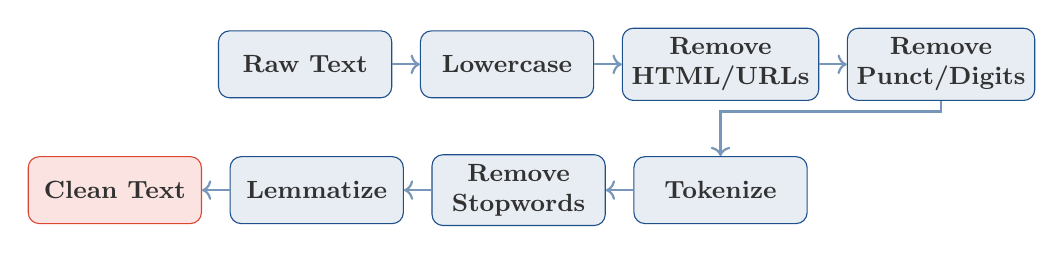
\begin{tikzpicture}[
  box/.style={draw=primary,fill=primary!10,rounded corners=4pt,minimum height=0.85cm,minimum width=2.2cm,font=\small\bfseries,align=center,text=darkgray},
  arrow/.style={->,thick,primary!60}
]
  \node[box] (raw)  {Raw Text};
  \node[box,right=0.35cm of raw]  (lc)  {Lowercase};
  \node[box,right=0.35cm of lc]   (rm)  {Remove\\HTML/URLs};
  \node[box,right=0.35cm of rm]   (rp)  {Remove\\Punct/Digits};
  \node[box,below=0.7cm of rm]    (tok) {Tokenize};
  \node[box,left=0.35cm of tok]   (sw)  {Remove\\Stopwords};
  \node[box,left=0.35cm of sw]    (lem) {Lemmatize};
  \node[box,left=0.35cm of lem,fill=accent!15,draw=accent] (out) {Clean Text};
  \draw[arrow] (raw) -- (lc);
  \draw[arrow] (lc) -- (rm);
  \draw[arrow] (rm) -- (rp);
  \draw[arrow] (rp) -- ++(0,-0.6) -| (tok);
  \draw[arrow] (tok) -- (sw);
  \draw[arrow] (sw) -- (lem);
  \draw[arrow] (lem) -- (out);
\end{tikzpicture}
\end{center}
\vspace{4pt}
\begin{columns}[T]
  \column{0.48\textwidth}
    \begin{block}{Steps Explained}
      \footnotesize
      \begin{itemize}
        \item \textbf{Lowercase}: Normalise case
        \item \textbf{Remove HTML/URLs}: Strip tags and links
        \item \textbf{Remove Punct/Digits}: Keep only alpha chars
        \item \textbf{Tokenize}: Split on whitespace
        \item \textbf{Stopwords}: sklearn's English list
        \item \textbf{Lemmatize}: Custom suffix-stripping rules (no NLTK)
      \end{itemize}
    \end{block}
  \column{0.48\textwidth}
    \begin{exampleblock}{Before \& After Example}
      \footnotesize
      \textbf{Before:}\\
      \textit{``Iraq's PM said the attack on Baghdad was..."}\\[4pt]
      \textbf{After:}\\
      \textit{``iraq prime minist attack baghdad"}
    \end{exampleblock}
    \begin{alertblock}{Why Lemmatize?}
      \footnotesize
      Reduces vocabulary: \textit{running, runs, ran} $\to$ \textit{run}. Less noise, better generalisation.
    \end{alertblock}
\end{columns}
\end{frame}

\section{Feature Engineering: TF-IDF}

%--- TF-IDF ---
\begin{frame}{TF-IDF Feature Engineering}
\begin{columns}[T]
  \column{0.50\textwidth}
    \begin{block}{TF-IDF Formula}
      \small
      \[
        \text{tfidf}(t,d) = \underbrace{\log(1+\text{tf}(t,d))}_{\text{Term Frequency}} \times \underbrace{\log\!\left(\tfrac{N}{1+\text{df}(t)}\right)}_{\text{Inverse Doc Freq}}
      \]
      \begin{itemize}\footnotesize
        \item \textbf{TF}: How often $t$ appears in doc $d$
        \item \textbf{IDF}: Penalises terms common across docs
        \item \textbf{sublinear\_tf}: log-dampens high-freq terms
      \end{itemize}
    \end{block}
    \vspace{4pt}
    \begin{tcolorbox}[colback=accent!8,colframe=accent,title=Vectoriser Settings,fonttitle=\footnotesize\bfseries]
      \footnotesize
      \begin{tabular}{ll}
        \texttt{max\_features} & 50,000 \\
        \texttt{ngram\_range}  & (1,\,2) --- unigrams + bigrams \\
        \texttt{sublinear\_tf} & True \\
        \texttt{min\_df}       & 2 (drop rare terms) \\
      \end{tabular}
    \end{tcolorbox}
  \column{0.47\textwidth}
    \begin{block}{Why TF-IDF for News?}
      \footnotesize
      \begin{itemize}
        \item Produces \textbf{sparse} high-dimensional vectors --- ideal for linear models
        \item \textbf{Bigrams} capture key phrases: \textit{``interest rate''}, \textit{``nuclear weapon''}
        \item Down-weights noise words like \textit{``said''} appearing across all categories
      \end{itemize}
    \end{block}
    \vspace{4pt}
    \begin{tcolorbox}[colback=light,colframe=primary,title=Matrix Properties,fonttitle=\footnotesize\bfseries]
      \footnotesize
      \begin{tabular}{ll}
        Train shape & $120{,}000 \times 50{,}000$ \\
        Test shape  & $7{,}600   \times 50{,}000$ \\
        Sparsity    & $\approx 99.8\%$ \\
      \end{tabular}
    \end{tcolorbox}
    \begin{tcolorbox}[colback=greencol!8,colframe=greencol,fonttitle=\footnotesize\bfseries,title=No Data Leakage!]
      \footnotesize
      TF-IDF fitted \textbf{only on train set}, then applied to test --- strictly correct ML practice.
    \end{tcolorbox}
\end{columns}
\end{frame}

\section{Models \& Methodology}

%--- Classifiers Overview ---
\begin{frame}{Classifier Models}
\begin{columns}[T]
  \column{0.24\textwidth}
    \begin{tcolorbox}[colback=worldcol!10,colframe=worldcol,title=Logistic Regression,fonttitle=\tiny\bfseries,height=7cm]
      \tiny
      \textbf{Concept:} Models $P(y|x)$ via softmax.\\[3pt]
      \textbf{Prediction:}
      \[p_k = \frac{e^{w_k^T x}}{\sum_j e^{w_j^T x}}\]
      \textbf{Settings:}\\
      $C=5$, solver=SAGA\\[3pt]
      \textbf{Strengths:}\\
      Fast, interpretable, strong baseline for sparse TF-IDF. L2 regularisation prevents overfitting.
    \end{tcolorbox}
  \column{0.24\textwidth}
    \begin{tcolorbox}[colback=sportscol!10,colframe=sportscol,title=Linear SVM,fonttitle=\tiny\bfseries,height=7cm]
      \tiny
      \textbf{Concept:} Max-margin hyperplane.\\[3pt]
      \textbf{Objective:}
      \[\min_w \tfrac{1}{2}\|w\|^2 + C\sum_i \xi_i\]
      \textbf{Settings:}\\
      $C=1.0$, LinearSVC\\[3pt]
      \textbf{Strengths:}\\
      Gold standard for text classification --- excellent on sparse high-dimensional data. OvA strategy for multiclass.
    \end{tcolorbox}
  \column{0.24\textwidth}
    \begin{tcolorbox}[colback=businesscol!10,colframe=businesscol,title=Random Forest,fonttitle=\tiny\bfseries,height=7cm]
      \tiny
      \textbf{Concept:} Bagged ensemble of decision trees.\\[3pt]
      \textbf{Prediction:}\\
      Majority vote of $T$ trees using random feature subsets\\[3pt]
      \textbf{Settings:}\\
      300 trees, n\_jobs=$-1$\\[3pt]
      \textbf{Weakness:}\\
      Struggles on very sparse high-dim data like TF-IDF
    \end{tcolorbox}
  \column{0.24\textwidth}
    \begin{tcolorbox}[colback=scitechcol!10,colframe=scitechcol,title=MLP Neural Net,fonttitle=\tiny\bfseries,height=7cm]
      \tiny
      \textbf{Concept:} Feedforward network.\\[3pt]
      \textbf{Architecture:}\\
      \texttt{50K$\to$256$\to$128$\to$64$\to$4}\\
      ReLU activations\\[3pt]
      \textbf{Settings:}\\
      Adam, L2 ($\alpha{=}0.0001$)\\
      50 epochs, early stopping (patience=5)\\[3pt]
      \textbf{Strengths:}\\
      Learns complex feature interactions
    \end{tcolorbox}
\end{columns}
\end{frame}

%--- MLP Architecture ---
\begin{frame}{MLP Neural Network --- Architecture}
\begin{center}
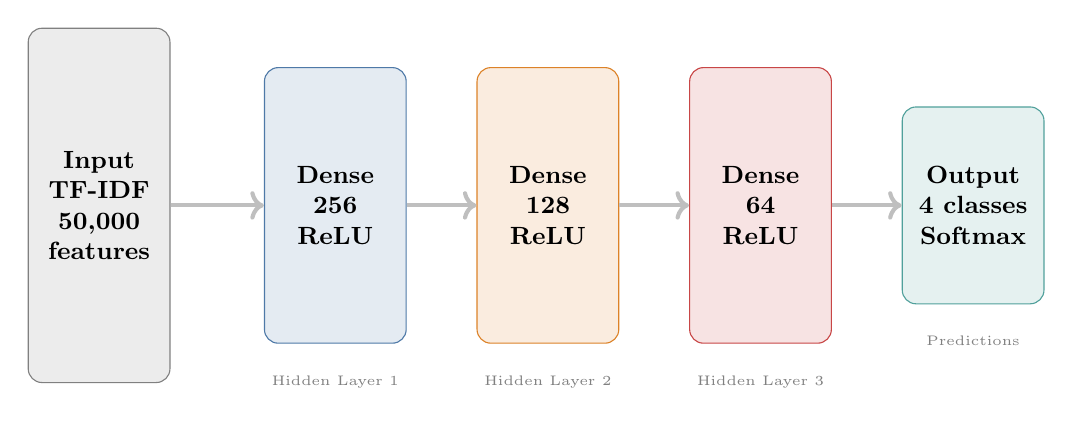
\begin{tikzpicture}[
  arrow/.style={->,thick,gray!50,line width=1.5pt}
]
  \node[mlplayer=gray,minimum height=4.5cm] (inp) at (0,0) {Input\\TF-IDF\\50{,}000\\features};
  \node[mlplayer=worldcol]   (h1) at (3.0,0) {Dense\\256\\ReLU};
  \node[mlplayer=sportscol]  (h2) at (5.7,0) {Dense\\128\\ReLU};
  \node[mlplayer=businesscol](h3) at (8.4,0) {Dense\\64\\ReLU};
  \node[mlplayer=scitechcol,minimum height=2.5cm] (out) at (11.1,0) {Output\\4 classes\\Softmax};
  \draw[arrow] (inp) -- (h1);
  \draw[arrow] (h1) -- (h2);
  \draw[arrow] (h2) -- (h3);
  \draw[arrow] (h3) -- (out);
  \node[below=8pt of h1,font=\tiny,gray] {Hidden Layer 1};
  \node[below=8pt of h2,font=\tiny,gray] {Hidden Layer 2};
  \node[below=8pt of h3,font=\tiny,gray] {Hidden Layer 3};
  \node[below=8pt of out,font=\tiny,gray] {Predictions};
\end{tikzpicture}
\end{center}
\vspace{4pt}
\begin{columns}
  \column{0.32\textwidth}
    \begin{tcolorbox}[colback=light,colframe=primary,title=Training Config,fonttitle=\footnotesize\bfseries]
      \footnotesize
      \textbf{Optimiser:} Adam\\
      \textbf{L2 reg:} $\alpha=0.0001$\\
      \textbf{Max epochs:} 50\\
      \textbf{Early stopping:} patience=5
    \end{tcolorbox}
  \column{0.32\textwidth}
    \begin{tcolorbox}[colback=light,colframe=primary,title=Why ReLU?,fonttitle=\footnotesize\bfseries]
      \footnotesize
      $\text{ReLU}(x) = \max(0,x)$\\[3pt]
      Avoids vanishing gradient. Sparse activations are efficient on high-dim TF-IDF input.
    \end{tcolorbox}
  \column{0.32\textwidth}
    \begin{tcolorbox}[colback=accent!8,colframe=accent,title=Early Stopping,fonttitle=\footnotesize\bfseries]
      \footnotesize
      Monitors 10\% validation split. Halts if no improvement for 5 consecutive epochs --- prevents overfitting.
    \end{tcolorbox}
\end{columns}
\end{frame}

\section{Exploratory Analysis}

%--- Keywords ---
\begin{frame}{Top Keywords per Category}
\begin{columns}[T]
  \column{0.50\textwidth}
    \begin{tcolorbox}[colback=worldcol!8,colframe=worldcol,title=World --- Top Terms,fonttitle=\footnotesize\bfseries]
      \footnotesize
      \textbf{said}, \textbf{iraq}, \textbf{reuter}, afp, kill, president, minist, new, people, govern\\[3pt]
      \textit{\scriptsize Dominated by geopolitical and conflict vocabulary}
    \end{tcolorbox}
    \vspace{4pt}
    \begin{tcolorbox}[colback=businesscol!8,colframe=businesscol,title=Business --- Top Terms,fonttitle=\footnotesize\bfseries]
      \footnotesize
      \textbf{said}, \textbf{reuter}, \textbf{new}, oil, company, stock, prices, percent, year, york\\[3pt]
      \textit{\scriptsize Financial and market-driven vocabulary}
    \end{tcolorbox}
  \column{0.47\textwidth}
    \begin{tcolorbox}[colback=sportscol!8,colframe=sportscol,title=Sports --- Top Terms,fonttitle=\footnotesize\bfseries]
      \footnotesize
      \textbf{game}, \textbf{win}, \textbf{team}, season, night, play, victory, year, cup, world\\[3pt]
      \textit{\scriptsize Highly distinctive competition vocabulary}
    \end{tcolorbox}
    \vspace{4pt}
    \begin{tcolorbox}[colback=scitechcol!8,colframe=scitechcol,title=Sci/Tech --- Top Terms,fonttitle=\footnotesize\bfseries]
      \footnotesize
      \textbf{new}, \textbf{microsoft}, \textbf{company}, software, internet, space, quot, comput, search\\[3pt]
      \textit{\scriptsize Technology-company and innovation vocabulary}
    \end{tcolorbox}
    \vspace{4pt}
    \begin{tcolorbox}[colback=accent!8,colframe=accent,fonttitle=\footnotesize\bfseries,title=Key Observation]
      \scriptsize
      \textbf{said} and \textbf{reuter} appear across all categories --- discriminating features must be content-specific terms.
    \end{tcolorbox}
\end{columns}
\end{frame}

%--- Word Clouds ---
\begin{frame}{Word Clouds per Category}
\begin{center}
  
\includegraphics[width=0.92\textwidth]{../outputs/wordclouds.png}
\end{center}
\vspace{-4pt}
\footnotesize\textit{Visually confirms distinct vocabulary per category --- strong separability supports high classification accuracy. Sports and Sci/Tech are the most visually distinctive.}
\end{frame}

\section{Results \& Evaluation}

%--- Dashboard ---
\begin{frame}{Full Results Dashboard}
\begin{center}
  
\includegraphics[width=0.93\textwidth]{../outputs/results_dashboard.png}
\end{center}
\end{frame}

%--- Accuracy ---
\begin{frame}{Model Accuracy Comparison}
\begin{columns}[T]
  \column{0.55\textwidth}
    \begin{center}
    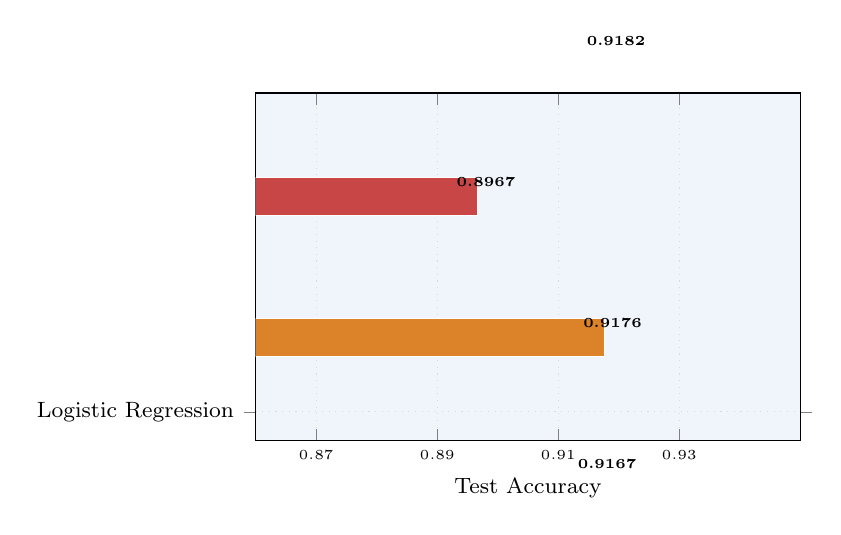
\begin{tikzpicture}
      \begin{axis}[
        xbar, bar width=14pt,
        width=8.5cm, height=6cm,
        symbolic y coords={{Logistic Regression},{Linear SVM},{Random Forest},{MLP Neural Network}},
        ytick=data,
        yticklabel style={font=\footnotesize},
        xmin=0.86, xmax=0.95,
        xtick={0.87,0.89,0.91,0.93},
        xticklabel style={font=\tiny},
        xlabel={Test Accuracy},
        xlabel style={font=\footnotesize},
        nodes near coords,
        nodes near coords style={font=\tiny\bfseries,xshift=3pt},
        nodes near coords align={horizontal},
        point meta=explicit symbolic,
        grid=major, grid style={dotted,gray!30},
        axis background/.style={fill=light},
      ]
        \addplot[fill=worldcol,draw=white] coordinates {(0.9167,{Logistic Regression}) [0.9167]};
        \addplot[fill=sportscol,draw=white] coordinates {(0.9176,{Linear SVM}) [0.9176]};
        \addplot[fill=businesscol,draw=white] coordinates {(0.8967,{Random Forest}) [0.8967]};
        \addplot[fill=scitechcol,draw=white] coordinates {(0.9182,{MLP Neural Network}) [0.9182]};
      \end{axis}
    \end{tikzpicture}
    \end{center}
  \column{0.42\textwidth}
    \begin{block}{Key Observations}
      \footnotesize
      \begin{itemize}
        \item \highlight{MLP} tops at \highlight{91.82\%} --- learns feature interactions
        \item \highlight{Linear SVM} close second (91.76\%) with faster training
        \item \highlight{Logistic Regression} competitive at 91.67\%
        \item \highlight{Random Forest} weakest (89.67\%) --- tree splits are inefficient on sparse data
      \end{itemize}
    \end{block}
    \vspace{4pt}
    \begin{tcolorbox}[colback=scitechcol!15,colframe=scitechcol,fonttitle=\footnotesize\bfseries,title=Winner]
      \centering\small MLP Neural Network\\
      \large\textbf{91.82\%} test accuracy
    \end{tcolorbox}
\end{columns}
\end{frame}

%--- F1 Heatmap ---
\begin{frame}{Per-Class F1-Score Heatmap}
\begin{columns}[T]
  \column{0.58\textwidth}
    \begin{center}
    \small\textbf{F1-Score Heatmap --- All Models}\\[6pt]
    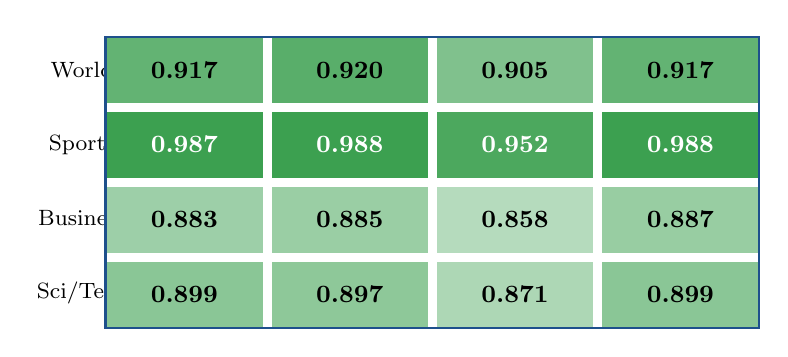
\begin{tikzpicture}[
      cell/.style={minimum width=2.0cm,minimum height=0.85cm,draw=white,align=center,font=\small\bfseries}
    ]
      % Column headers (no foreach - avoids beamer parameter error)
      \node[font=\footnotesize\bfseries,primary] at (1.05,3.6) {LR};
      \node[font=\footnotesize\bfseries,primary] at (3.15,3.6) {SVM};
      \node[font=\footnotesize\bfseries,primary] at (5.25,3.6) {RF};
      \node[font=\footnotesize\bfseries,primary] at (7.35,3.6) {MLP};
      % Row headers (Sci/Tech slash must NOT be used as foreach separator)
      \node[font=\footnotesize,align=right] at (-0.3,0.45)  {Sci/Tech};
      \node[font=\footnotesize,align=right] at (-0.3,1.40)  {Business};
      \node[font=\footnotesize,align=right] at (-0.3,2.325) {Sports};
      \node[font=\footnotesize,align=right] at (-0.3,3.275) {World};
      % World row (explicit cells - no foreach)
      \fill[greencol!80] (0.0,2.85) rectangle ++(2.0,0.85); \node[cell] at (1.0,3.275) {0.917};
      \fill[greencol!85] (2.1,2.85) rectangle ++(2.0,0.85); \node[cell] at (3.1,3.275) {0.920};
      \fill[greencol!65] (4.2,2.85) rectangle ++(2.0,0.85); \node[cell] at (5.2,3.275) {0.905};
      \fill[greencol!80] (6.3,2.85) rectangle ++(2.0,0.85); \node[cell] at (7.3,3.275) {0.917};
      % Sports row
      \fill[greencol]    (0.0,1.90) rectangle ++(2.0,0.85); \node[cell,white] at (1.0,2.325) {0.987};
      \fill[greencol]    (2.1,1.90) rectangle ++(2.0,0.85); \node[cell,white] at (3.1,2.325) {0.988};
      \fill[greencol!92] (4.2,1.90) rectangle ++(2.0,0.85); \node[cell,white] at (5.2,2.325) {0.952};
      \fill[greencol]    (6.3,1.90) rectangle ++(2.0,0.85); \node[cell,white] at (7.3,2.325) {0.988};
      % Business row
      \fill[greencol!50] (0.0,0.95) rectangle ++(2.0,0.85); \node[cell] at (1.0,1.375) {0.883};
      \fill[greencol!52] (2.1,0.95) rectangle ++(2.0,0.85); \node[cell] at (3.1,1.375) {0.885};
      \fill[greencol!38] (4.2,0.95) rectangle ++(2.0,0.85); \node[cell] at (5.2,1.375) {0.858};
      \fill[greencol!53] (6.3,0.95) rectangle ++(2.0,0.85); \node[cell] at (7.3,1.375) {0.887};
      % SciTech row
      \fill[greencol!60] (0.0,0.00) rectangle ++(2.0,0.85); \node[cell] at (1.0,0.425) {0.899};
      \fill[greencol!58] (2.1,0.00) rectangle ++(2.0,0.85); \node[cell] at (3.1,0.425) {0.897};
      \fill[greencol!42] (4.2,0.00) rectangle ++(2.0,0.85); \node[cell] at (5.2,0.425) {0.871};
      \fill[greencol!60] (6.3,0.00) rectangle ++(2.0,0.85); \node[cell] at (7.3,0.425) {0.899};
      \draw[primary,thick] (0,0) rectangle (8.3,3.7);
    \end{tikzpicture}
    \end{center}
  \column{0.39\textwidth}
    \begin{block}{Insights}
      \footnotesize
      \begin{itemize}
        \item \textbf{Sports} F1 $\approx$0.987 --- very distinctive vocabulary
        \item \textbf{Business} hardest ($\approx$0.85--0.89) --- overlaps with World and Sci/Tech
        \item \textbf{Linear models} consistently outperform Random Forest
        \item \textbf{MLP} matches or beats all classicals
      \end{itemize}
    \end{block}
    \vspace{4pt}
    \begin{alertblock}{Why is Business Hardest?}
      \footnotesize
      Business articles mention tech companies ($\to$ Sci/Tech confusion) and world events like oil/geopolitics ($\to$ World confusion)
    \end{alertblock}
\end{columns}
\end{frame}

%--- Confusion Matrix ---
\begin{frame}{Confusion Matrix --- MLP Neural Network}
\begin{columns}[T]
  \column{0.52\textwidth}
    \begin{center}
    \small\textbf{MLP Neural Network --- Test Set (7,600 articles)}\\[6pt]
    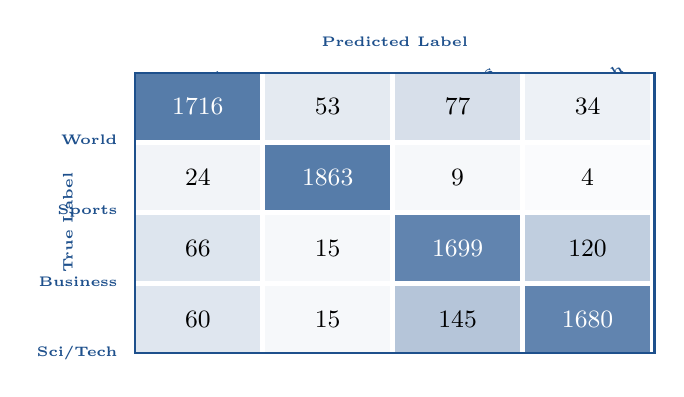
\begin{tikzpicture}[
      cell/.style={minimum width=1.6cm,minimum height=0.85cm,draw=white,align=center,font=\small},
      hdr/.style={font=\tiny\bfseries,primary}
    ]
      % Column and row headers (no foreach to avoid beamer parameter error)
      \node[hdr,rotate=30] at (0.8,3.8)  {World};
      \node[hdr,rotate=30] at (2.45,3.8) {Sports};
      \node[hdr,rotate=30] at (4.10,3.8) {Business};
      \node[hdr,rotate=30] at (5.75,3.8) {Sci/Tech};
      \node[hdr,anchor=east] at (-0.1,0.45)  {Sci/Tech};
      \node[hdr,anchor=east] at (-0.1,1.35)  {Business};
      \node[hdr,anchor=east] at (-0.1,2.25)  {Sports};
      \node[hdr,anchor=east] at (-0.1,3.15)  {World};
      % World row
      \fill[primary!75] (0,3.15) rectangle ++(1.6,0.85);
      \fill[primary!12] (1.65,3.15) rectangle ++(1.6,0.85);
      \fill[primary!18] (3.30,3.15) rectangle ++(1.6,0.85);
      \fill[primary!8]  (4.95,3.15) rectangle ++(1.6,0.85);
      \node[cell,white] at (0.8,3.575) {1716};
      \node[cell] at (2.45,3.575) {53};
      \node[cell] at (4.10,3.575) {77};
      \node[cell] at (5.75,3.575) {34};
      % Sports row
      \fill[primary!6]  (0,2.25) rectangle ++(1.6,0.85);
      \fill[primary!75] (1.65,2.25) rectangle ++(1.6,0.85);
      \fill[primary!4]  (3.30,2.25) rectangle ++(1.6,0.85);
      \fill[primary!2]  (4.95,2.25) rectangle ++(1.6,0.85);
      \node[cell] at (0.8,2.675) {24};
      \node[cell,white] at (2.45,2.675) {1863};
      \node[cell] at (4.10,2.675) {9};
      \node[cell] at (5.75,2.675) {4};
      % Business row
      \fill[primary!15] (0,1.35) rectangle ++(1.6,0.85);
      \fill[primary!4]  (1.65,1.35) rectangle ++(1.6,0.85);
      \fill[primary!70] (3.30,1.35) rectangle ++(1.6,0.85);
      \fill[primary!28] (4.95,1.35) rectangle ++(1.6,0.85);
      \node[cell] at (0.8,1.775) {66};
      \node[cell] at (2.45,1.775) {15};
      \node[cell,white] at (4.10,1.775) {1699};
      \node[cell] at (5.75,1.775) {120};
      % SciTech row
      \fill[primary!14] (0,0.45) rectangle ++(1.6,0.85);
      \fill[primary!4]  (1.65,0.45) rectangle ++(1.6,0.85);
      \fill[primary!33] (3.30,0.45) rectangle ++(1.6,0.85);
      \fill[primary!70] (4.95,0.45) rectangle ++(1.6,0.85);
      \node[cell] at (0.8,0.875) {60};
      \node[cell] at (2.45,0.875) {15};
      \node[cell] at (4.10,0.875) {145};
      \node[cell,white] at (5.75,0.875) {1680};
      \draw[primary,thick] (0,0.45) rectangle (6.6,4.0);
      \node[hdr,rotate=90,anchor=center] at (-0.85,2.1) {True Label};
      \node[hdr] at (3.3,4.4) {Predicted Label};
    \end{tikzpicture}
    \end{center}
  \column{0.45\textwidth}
    \begin{block}{Error Analysis}
      \footnotesize
      \begin{itemize}
        \item \textbf{Sports} cleanest: only 37 misclassifications from 1,900
        \item \textbf{Business$\to$Sci/Tech}: 120 errors --- tech companies in business news
        \item \textbf{Sci/Tech$\to$Business}: 145 errors --- financial tech articles
        \item \textbf{World} modest confusion with Business/Sci/Tech
      \end{itemize}
    \end{block}
    \vspace{4pt}
    \begin{tcolorbox}[colback=light,colframe=primary,title=Per-Class Accuracy,fonttitle=\footnotesize\bfseries]
      \footnotesize
      \begin{tabular}{lr}
        World    & 90.3\% \\
        Sports   & \textbf{98.0\%} \\
        Business & 89.4\% \\
        Sci/Tech & 88.4\% \\
      \end{tabular}
    \end{tcolorbox}
\end{columns}
\end{frame}

%--- Cross-Validation ---
\begin{frame}{5-Fold Cross-Validation}
\begin{columns}[T]
  \column{0.55\textwidth}
    \begin{center}
    \textbf{CV Results --- Logistic Regression}\\[4pt]
    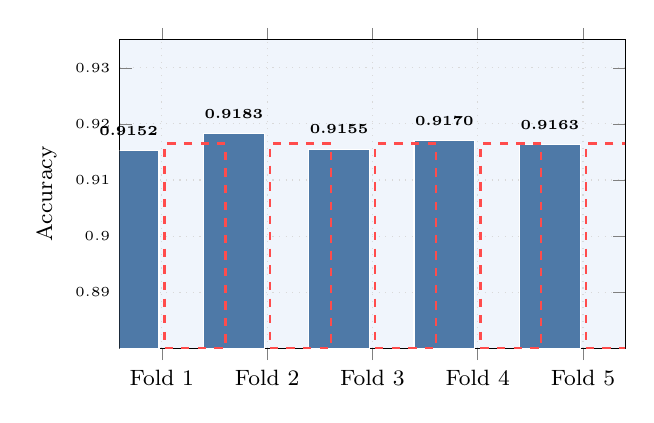
\begin{tikzpicture}
      \begin{axis}[
        ybar, bar width=22pt,
        width=8cm, height=5.5cm,
        symbolic x coords={{Fold 1},{Fold 2},{Fold 3},{Fold 4},{Fold 5}},
        xtick=data,
        xticklabel style={font=\footnotesize},
        ymin=0.88, ymax=0.935,
        ytick={0.89,0.90,0.91,0.92,0.93},
        yticklabel style={font=\tiny},
        ylabel={Accuracy},
        ylabel style={font=\footnotesize},
        nodes near coords,
        nodes near coords style={font=\tiny\bfseries,yshift=2pt},
        point meta=explicit symbolic,
        grid=major, grid style={dotted,gray!30},
        axis background/.style={fill=light},
      ]
        \addplot[fill=worldcol,draw=white] coordinates {
          ({Fold 1},0.9152) [0.9152]
          ({Fold 2},0.9183) [0.9183]
          ({Fold 3},0.9155) [0.9155]
          ({Fold 4},0.9170) [0.9170]
          ({Fold 5},0.9163) [0.9163]
        };
        \addplot[no marks,red!70,thick,dashed] coordinates {
          ({Fold 1},0.9165) ({Fold 2},0.9165) ({Fold 3},0.9165)
          ({Fold 4},0.9165) ({Fold 5},0.9165)
        };
      \end{axis}
    \end{tikzpicture}\\
    \small\textbf{Mean: 0.9165 $\pm$ 0.0011} (5-fold, 24K subsample)
    \end{center}
  \column{0.42\textwidth}
    \begin{block}{What Cross-Validation Tells Us}
      \footnotesize
      \begin{itemize}
        \item Very \textbf{low variance} ($\pm$0.0011) --- model is stable
        \item Results are \textbf{not a lucky split}
        \item Mean CV $\approx$ test accuracy: \textbf{no overfitting}
      \end{itemize}
    \end{block}
    \vspace{4pt}
    \begin{exampleblock}{K-Fold CV Method}
      \footnotesize
      Data split into $k{=}5$ equal folds. Each fold acts as validation once; model trained on remaining 4. Final score = mean of 5 validation accuracies.
    \end{exampleblock}
    \vspace{4pt}
    \begin{tcolorbox}[colback=greencol!8,colframe=greencol,fonttitle=\footnotesize\bfseries,title=Stability Confirmed]
      \footnotesize
      Standard deviation of 0.0011 indicates the pipeline generalises well regardless of the random data split.
    \end{tcolorbox}
\end{columns}
\end{frame}

\section{Summary \& Conclusions}

%--- Summary Table ---
\begin{frame}{Results Summary}
\begin{center}
\begin{tcolorbox}[colback=light,colframe=primary,title=\textbf{Final Model Comparison --- AG News Test Set (7,600 articles)},fonttitle=\normalsize\bfseries,width=\textwidth]
  \centering\small
  \setlength{\tabcolsep}{6pt}
  \begin{tabular}{lccccc}
    \toprule
    \textbf{Model} & \textbf{Accuracy} & \textbf{World F1} & \textbf{Sports F1} & \textbf{Business F1} & \textbf{Sci/Tech F1}\\
    \midrule
    \rowcolor{worldcol!20}
    Logistic Regression & 0.9167 & 0.917 & 0.987 & 0.883 & 0.899\\
    \rowcolor{sportscol!20}
    Linear SVM          & 0.9176 & 0.920 & 0.988 & 0.885 & 0.897\\
    \rowcolor{businesscol!20}
    Random Forest       & 0.8967 & 0.905 & 0.952 & 0.858 & 0.871\\
    \rowcolor{scitechcol!30}
    \textbf{MLP Neural Network} & \textbf{0.9182} & \textbf{0.917} & \textbf{0.988} & \textbf{0.887} & \textbf{0.899}\\
    \bottomrule
  \end{tabular}
\end{tcolorbox}
\end{center}
\vspace{4pt}
\begin{columns}
  \column{0.32\textwidth}
    \begin{tcolorbox}[colback=scitechcol!15,colframe=scitechcol,fonttitle=\footnotesize\bfseries,title=Best Overall]
      \centering\small MLP Neural Network\\91.82\% accuracy
    \end{tcolorbox}
  \column{0.32\textwidth}
    \begin{tcolorbox}[colback=sportscol!15,colframe=sportscol,fonttitle=\footnotesize\bfseries,title=Best Efficiency]
      \centering\small Linear SVM\\91.76\% --- fastest training
    \end{tcolorbox}
  \column{0.32\textwidth}
    \begin{tcolorbox}[colback=businesscol!15,colframe=businesscol,fonttitle=\footnotesize\bfseries,title=Weakest]
      \centering\small Random Forest\\89.67\% --- sparse data issues
    \end{tcolorbox}
\end{columns}
\end{frame}

%--- Takeaways ---
\begin{frame}{Key Takeaways \& Conclusions}
\begin{columns}[T]
  \column{0.50\textwidth}
    \begin{block}{What Worked Well}
      \small
      \begin{enumerate}
        \item \textbf{TF-IDF + Linear models} are extremely effective --- simple, fast, accurate
        \item \textbf{Bigrams} captured key phrases: \textit{``interest rate''}, \textit{``oil price''}
        \item \textbf{Balanced dataset} (30K/class) eliminated class bias
        \item \textbf{MLP} outperforms all classicals with simple 3-layer architecture
        \item \textbf{Cross-validation} confirmed robustness --- results are not chance
      \end{enumerate}
    \end{block}
  \column{0.47\textwidth}
    \begin{block}{Lessons Learned}
      \small
      \begin{itemize}
        \item Business/Sci/Tech boundary is inherently ambiguous
        \item Sports is most distinguishable --- unique lexicon
        \item Random Forests struggle on sparse TF-IDF vectors
        \item Linear models remain very competitive with neural nets on text
      \end{itemize}
    \end{block}
    \vspace{4pt}
    \begin{tcolorbox}[colback=accent!8,colframe=accent,title=Future Directions,fonttitle=\footnotesize\bfseries]
      \footnotesize
      \begin{itemize}
        \item \textbf{BERT/DistilBERT} fine-tuning ($>$95\% expected)
        \item Hyperparameter tuning (GridSearchCV)
        \item Character-level n-grams for robustness
        \item Attention-based feature importance analysis
      \end{itemize}
    \end{tcolorbox}
\end{columns}
\end{frame}

%--- Final ---
\begin{frame}[plain]
\begin{tikzpicture}[remember picture,overlay]
  \fill[primary] (current page.north west) rectangle (current page.south east);
  \filldraw[white,opacity=0.04] (current page.center) circle (6cm);
  \fill[worldcol]    ([yshift=0.55cm]current page.south west) rectangle ++(0.25\paperwidth,0.55cm);
  \fill[sportscol]   ([yshift=0.55cm,xshift=0.25\paperwidth]current page.south west) rectangle ++(0.25\paperwidth,0.55cm);
  \fill[businesscol] ([yshift=0.55cm,xshift=0.50\paperwidth]current page.south west) rectangle ++(0.25\paperwidth,0.55cm);
  \fill[scitechcol]  ([yshift=0.55cm,xshift=0.75\paperwidth]current page.south west) rectangle ++(0.25\paperwidth,0.55cm);
  \node[white,font=\small\bfseries] at ([yshift=0.825cm,xshift=0.125\paperwidth]current page.south west) {World};
  \node[white,font=\small\bfseries] at ([yshift=0.825cm,xshift=0.375\paperwidth]current page.south west) {Sports};
  \node[white,font=\small\bfseries] at ([yshift=0.825cm,xshift=0.625\paperwidth]current page.south west) {Business};
  \node[white,font=\small\bfseries] at ([yshift=0.825cm,xshift=0.875\paperwidth]current page.south west) {Sci/Tech};
  \node[white,font=\Huge\bfseries] at ([yshift=1.2cm]current page.center) {Thank You};
  \node[white!70,font=\large,text width=12cm,align=center] at ([yshift=0.2cm]current page.center) {News Category Classification on AG News};
  \node[white!50,font=\normalsize,text width=14cm,align=center] at ([yshift=-0.8cm]current page.center) {MLP: \textbf{91.82\%} $\cdot$ Linear SVM: \textbf{91.76\%} $\cdot$ Logistic Regression: \textbf{91.67\%} $\cdot$ Random Forest: \textbf{89.67\%}};
  \node[white!40,font=\small,text width=14cm,align=center] at ([yshift=-1.6cm]current page.center) {TF-IDF (50K features, unigrams + bigrams) $\cdot$ 120{,}000 training articles $\cdot$ 4 balanced categories};
\end{tikzpicture}
\end{frame}

\end{document}